% ============================================================
\chapter{Optimality Conditions --- KKT}
\label{ch:kkt}
% ============================================================

In unconstrained optimisation, the optimality condition is simple: the gradient vanishes. But as soon as constraints are added---inequalities, equalities---this na\"ive condition no longer suffices. The Karush-Kuhn-Tucker (KKT) conditions, discovered independently by William Karush in 1939 (in a master's thesis that remained long ignored) and by Harold Kuhn and Albert Tucker in 1951, generalise the zero-gradient condition by introducing \emph{Lagrange multipliers} for the constraints. In convex optimisation, under very general constraint qualifications, KKT conditions are not only necessary but also \emph{sufficient}---they completely characterise optimal solutions.

\section{Introduction}

The Karush--Kuhn--Tucker (KKT) conditions generalize the classical condition
$\nabla f(x^*) = 0$ to constrained optimization problems. In convex optimization,
under very general constraint qualifications, the KKT conditions are both necessary
and sufficient for optimality.

\section{Constrained Convex Optimization Problem}

Consider the general problem:
\[
    \begin{aligned}
        & \min_{x \in \R^n} && f(x) \\
        & \text{subject to} && g_i(x) \leq 0, \quad i = 1, \ldots, m, \\
        & && h_j(x) = 0, \quad j = 1, \ldots, p,
    \end{aligned}
    \tag{P}
\]
where $f$ and the $g_i$ are convex and the $h_j$ are affine: $h_j(x) = a_j^T x - b_j$.

\begin{definition}[Feasible Set]
The \emph{feasible set} is:
\[
    \mathcal{F} = \{x \in \R^n \mid g_i(x) \leq 0, \; i=1,\ldots,m, \;
    h_j(x) = 0, \; j=1,\ldots,p\}.
\]
\end{definition}

\begin{definition}[Active Constraint]
The constraint $g_i(x) \leq 0$ is \emph{active} at $x$ if $g_i(x) = 0$. The active
index set is $\mathcal{A}(x) = \{i \mid g_i(x) = 0\}$.
\end{definition}

\section{KKT Conditions}

\begin{definition}[KKT Conditions]
A point $x^* \in \mathcal{F}$ satisfies the \emph{KKT conditions} if there exist
multipliers $\lambda^* \in \R^m$ and $\nu^* \in \R^p$ such that:
\begin{enumerate}
    \item \textbf{Stationarity}:
    $\displaystyle 0 \in \partial f(x^*) + \sum_{i=1}^m \lambda_i^* \partial g_i(x^*)
    + \sum_{j=1}^p \nu_j^* a_j$.
    \item \textbf{Primal feasibility}: $g_i(x^*) \leq 0$ and $h_j(x^*) = 0$.
    \item \textbf{Dual feasibility}: $\lambda_i^* \geq 0$ for all $i$.
    \item \textbf{Complementary slackness}: $\lambda_i^* g_i(x^*) = 0$ for all $i$.
\end{enumerate}
\end{definition}

If $f$ and the $g_i$ are differentiable, the stationarity condition reads:
\[
    \nabla f(x^*) + \sum_{i=1}^m \lambda_i^* \nabla g_i(x^*) + \sum_{j=1}^p \nu_j^* a_j = 0.
\]

\begin{keyformulas}[title=\textbf{KKT Conditions (Differentiable Case)}]
\[
    \nabla f(x^*) + \sum_{i=1}^m \lambda_i^* \nabla g_i(x^*) + A^T\nu^* = 0, \quad
    \lambda^* \geq 0, \quad
    \lambda^* \circ g(x^*) = 0, \quad
    g(x^*) \leq 0, \quad
    Ax^* = b.
\]
\end{keyformulas}

\begin{intuition}
The complementary slackness condition $\lambda_i^* g_i(x^*) = 0$ means that either
the constraint is inactive ($g_i(x^*) < 0$ and $\lambda_i^* = 0$) or it is active
($g_i(x^*) = 0$ and $\lambda_i^* \geq 0$ potentially nonzero). The multiplier
$\lambda_i^*$ measures the ``force'' with which the constraint pushes the solution.
\end{intuition}

\section{Constraint Qualifications}

\begin{definition}[Slater's Condition]
\emph{Slater's condition} is satisfied if there exists a strictly feasible point
$\hat{x}$ such that:
\[
    g_i(\hat{x}) < 0, \quad i = 1, \ldots, m, \quad
    h_j(\hat{x}) = 0, \quad j = 1, \ldots, p.
\]
(For affine constraints $g_i$, it suffices that $g_i(\hat{x}) \leq 0$.)
\end{definition}

\begin{theorem}[KKT --- Necessary and Sufficient Conditions]
\label{thm:kkt}
Consider problem (P) with $f, g_i$ convex and $h_j$ affine.
\begin{enumerate}
    \item \textbf{Sufficiency (always)}: if $(x^*, \lambda^*, \nu^*)$ satisfies the
    KKT conditions, then $x^*$ is an optimal solution of (P).
    \item \textbf{Necessity (under Slater)}: if Slater's condition holds and $x^*$
    is optimal, then there exists $(\lambda^*, \nu^*)$ such that
    $(x^*, \lambda^*, \nu^*)$ satisfies the KKT conditions.
\end{enumerate}
\end{theorem}

\begin{proof}[Proof of sufficiency]
Suppose $(x^*, \lambda^*, \nu^*)$ satisfies KKT. For any $x \in \mathcal{F}$:
\begin{align*}
    f(x) &\geq f(x^*) + \inner{g_f}{x - x^*}
    \quad \text{where } g_f \in \partial f(x^*) \\
    &= f(x^*) - \sum_i \lambda_i^* \inner{g_{g_i}}{x-x^*} - \sum_j \nu_j^* a_j^T(x-x^*)
    \quad \text{(stationarity)} \\
    &\geq f(x^*) - \sum_i \lambda_i^*(g_i(x) - g_i(x^*)) - \sum_j \nu_j^*(h_j(x) - h_j(x^*))
    \quad \text{(subgradient of } g_i) \\
    &\geq f(x^*) - \sum_i \lambda_i^* g_i(x) + \sum_i \lambda_i^* g_i(x^*)
    \quad \text{(since } h_j(x) = h_j(x^*) = 0) \\
    &\geq f(x^*) \quad \text{(since } \lambda_i^* \geq 0, g_i(x) \leq 0,
    \lambda_i^* g_i(x^*) = 0).
\end{align*}
\end{proof}

\section{Examples of KKT Application}

\begin{example}[Quadratic Programming]
Consider:
\[
    \min_x \frac{1}{2}x^TQx + c^Tx \quad \text{subject to} \quad Ax \leq b.
\]
The KKT conditions are:
\[
    Qx^* + c + A^T\lambda^* = 0, \quad \lambda^* \geq 0, \quad
    Ax^* \leq b, \quad \lambda^* \circ (Ax^* - b) = 0.
\]
\end{example}

\begin{example}[Projection onto a Convex Set]
The projection $\bar{x} = \mathrm{proj}_C(y)$ solves:
\[
    \min_x \frac{1}{2}\norm{x - y}^2 \quad \text{subject to} \quad x \in C.
\]
If $C = \{x \mid g_i(x) \leq 0\}$, the KKT conditions give:
\[
    \bar{x} - y + \sum_i \lambda_i^* \nabla g_i(\bar{x}) = 0, \quad
    \lambda_i^* \geq 0, \quad \lambda_i^* g_i(\bar{x}) = 0.
\]
\end{example}

\begin{example}[Hard-Margin SVM]
The primal SVM:
\[
    \min_{w,b} \frac{1}{2}\norm{w}^2 \quad \text{subject to} \quad
    y_i(\inner{w}{x_i} + b) \geq 1, \; i=1,\ldots,N.
\]
The KKT conditions:
\[
    w^* = \sum_i \alpha_i^* y_i x_i, \quad
    \sum_i \alpha_i^* y_i = 0, \quad
    \alpha_i^* \geq 0, \quad
    \alpha_i^*(y_i(\inner{w^*}{x_i} + b^*) - 1) = 0.
\]
Complementary slackness shows that only points with
$y_i(\inner{w^*}{x_i} + b^*) = 1$ (support vectors) have $\alpha_i^* > 0$.
\end{example}

\section{Geometric Interpretation}

\begin{center}
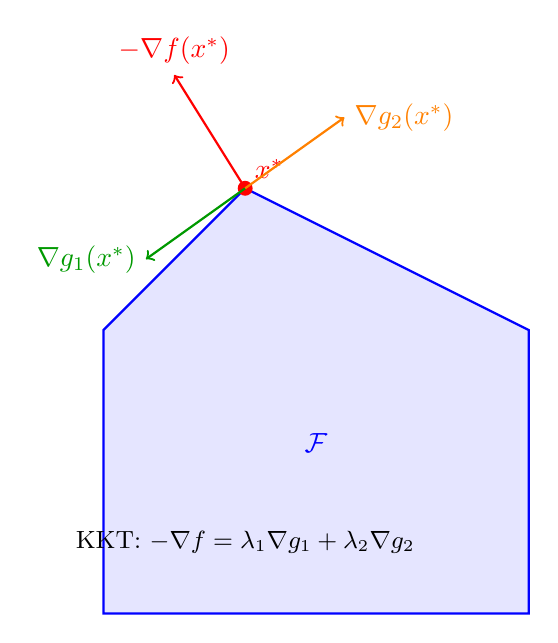
\begin{tikzpicture}[scale=1.8]
    % Feasible region
    \fill[blue!10] (0,0) -- (3,0) -- (3,2) -- (1,3) -- (0,2) -- cycle;
    \draw[thick, blue] (0,0) -- (3,0) -- (3,2) -- (1,3) -- (0,2) -- cycle;

    % Optimal point
    \fill[red] (1,3) circle (1.5pt) node[above right] {$x^*$};

    % Gradient of f
    \draw[->, thick, red] (1,3) -- (0.5,3.8) node[above] {$-\nabla f(x^*)$};

    % Constraint gradients
    \draw[->, thick, green!60!black] (1,3) -- (0.3,2.5) node[left] {$\nabla g_1(x^*)$};
    \draw[->, thick, orange] (1,3) -- (1.7,3.5) node[right] {$\nabla g_2(x^*)$};

    % Labels
    \node[blue] at (1.5,1.2) {$\mathcal{F}$};
    \node at (1, 0.5) {\small KKT: $-\nabla f = \lambda_1 \nabla g_1 + \lambda_2 \nabla g_2$};
\end{tikzpicture}
\end{center}

\section{Other Constraint Qualifications}

\begin{definition}[Linear Independence (LICQ)]
\emph{LICQ} holds at $x^*$ if the gradients of the active constraints
$\{\nabla g_i(x^*)\}_{i \in \mathcal{A}(x^*)} \cup \{a_j\}_{j=1}^p$ are linearly
independent.
\end{definition}

\begin{proposition}
Under LICQ, the KKT multipliers are unique.
\end{proposition}

\begin{definition}[Mangasarian--Fromovitz (MFCQ)]
\emph{MFCQ} holds at $x^*$ if the $\{a_j\}$ are linearly independent and there
exists $d \in \R^n$ such that:
\[
    \inner{\nabla g_i(x^*)}{d} < 0, \; \forall i \in \mathcal{A}(x^*), \quad
    a_j^T d = 0, \; \forall j.
\]
\end{definition}

\section{Sensitivity and Economic Interpretation}

\begin{theorem}[Sensitivity]
\label{thm:sensitivity}
Let $p^*(u, v)$ be the optimal value of the perturbed problem:
\[
    \min f(x) \quad \text{subject to} \quad g_i(x) \leq u_i, \; h_j(x) = v_j.
\]
Under regularity conditions, the KKT multipliers satisfy:
\[
    \lambda_i^* = -\frac{\partial p^*}{\partial u_i}\bigg|_{(0,0)}, \quad
    \nu_j^* = -\frac{\partial p^*}{\partial v_j}\bigg|_{(0,0)}.
\]
\end{theorem}

\begin{remark}
$\lambda_i^*$ represents the ``shadow price'' of the $i$-th constraint: relaxing the
constraint by one unit improves the optimal value by $\lambda_i^*$.
\end{remark}

\section{Python Implementation}

\begin{codeblock}[title=\textbf{Verifying KKT conditions with CVXPY}]
\begin{minted}{python}
import numpy as np
import cvxpy as cp

# Quadratic programming
n = 5
np.random.seed(42)
Q = np.random.randn(n, n)
Q = Q.T @ Q + 0.1 * np.eye(n)  # PD
c = np.random.randn(n)
A = np.random.randn(3, n)
b = np.ones(3)

x = cp.Variable(n)
constraints = [A @ x <= b]
prob = cp.Problem(cp.Minimize(0.5 * cp.quad_form(x, Q) + c @ x),
                  constraints)
prob.solve()

x_star = x.value
lambda_star = constraints[0].dual_value

print("Solution x*:", x_star)
print("Multipliers lambda*:", lambda_star)

# Verify stationarity
grad_L = Q @ x_star + c + A.T @ lambda_star
print(f"||grad L|| = {np.linalg.norm(grad_L):.2e}")

# Verify complementary slackness
slack = b - A @ x_star
comp = lambda_star * slack
print(f"Complementarity: max|lambda*g| = {np.max(np.abs(comp)):.2e}")

# Verify feasibility
print(f"Primal feasibility: max(Ax-b) = {np.max(A @ x_star - b):.2e}")
print(f"Dual feasibility: min(lambda) = {np.min(lambda_star):.2e}")
\end{minted}
\end{codeblock}

\section{Exercises}

\begin{exercise}[$\star$]
Solve $\min x_1^2 + x_2^2$ subject to $x_1 + x_2 \geq 1$ using the KKT conditions.
\end{exercise}

\begin{exercise}[$\star$]
Verify that Slater's condition holds for
$\min \norm{x}^2$ subject to $\norm{x}_\infty \leq 1$.
\end{exercise}

\begin{exercise}[$\star\star$]
Derive the KKT conditions for the soft-margin SVM problem:
\[
    \min_{w,b,\xi} \frac{1}{2}\norm{w}^2 + C\sum_i \xi_i \quad \text{subject to} \quad
    y_i(\inner{w}{x_i} + b) \geq 1 - \xi_i, \; \xi_i \geq 0.
\]
\end{exercise}

\begin{exercise}[$\star\star$]
Show that for a linear programming problem, the KKT conditions are equivalent to the
primal-dual complementarity conditions.
\end{exercise}

\begin{exercise}[$\star\star\star$]
Prove the sensitivity theorem~\ref{thm:sensitivity} for a linear programming problem.
\end{exercise}

\begin{exercise}[$\star\star\star$]
Show that under LICQ, the KKT multipliers are unique. Give an example where LICQ
fails and multipliers are not unique.
\end{exercise}
